\documentclass[10pt]{article}

\usepackage{amsmath}

\usepackage{amssymb}

\ifx\pdfoutput\undefined
  \usepackage[dvips]{graphicx}
\else
  \RequirePackage[pdftex]{graphicx}
\fi

%\usepackage{longtable}

\usepackage[small,bf]{caption}

\usepackage{array}



% Margin adjustments.  vmargin.sty interacts badly with page numbers at

% the bottom of the page, so we just code the number manually here.



\oddsidemargin  0pt

\evensidemargin 0pt

\ifx\pdfoutput\undefined
  \setlength{\topmargin}{1 ex}
\else
  \setlength{\topmargin}{-8 ex}
\fi

\hoffset        0 in

\textwidth      6.5 in

\textheight     9 in



% Style adjustments.



% Fix placement of figures & tables.  This keeps latex from shoving big

% floats to the end of a document when they are somewhat big, which it will

% do even if you put [htb] as the argument.



\setcounter{topnumber}{1}

\setcounter{bottomnumber}{1}

\def\topfraction{1.0}

\def\bottomfraction{1.0}

\def\textfraction{0.1}

\def\floatpagefraction{0.9}



\renewcommand{\arraystretch}{1.1}



%begin{latexonly}



\raggedbottom



\def\captionfont{\itshape}              % Use italic font for captions.



\makeatletter



\setlength{\parindent}{0 pt}            % Unindented paragraphs, separated ...

\setlength{\parskip}{1.3 ex}            % ... by roughly one blank line.

\setlength{\partopsep}{-1 ex}



\renewcommand{\section}{\@startsection%
  {section}{1}{0pt}{-1.8ex \@plus -1ex \@minus -.2ex}%
  {0.8ex}{\normalfont\Large\bfseries\sffamily}}



\renewcommand{\subsection}{\@startsection%
  {subsection}{2}{0pt}{-2ex \@plus 1ex \@minus -.2ex}%
  {0.8ex}{\slshape\large\bfseries\sffamily}}



\renewcommand{\subsubsection}{\@startsection%
  {subsubsection}{3}{0pt}{-1.5ex \@plus 1ex \@minus -.2ex}%
  {0.5ex}{\slshape\normalsize\bfseries\sffamily}}



% The following is a modified version of the macro from article.cls.

% It adjusts the vertical spacing in TOC for section lines.



\renewcommand*\l@section[2]{%
  \ifnum \c@tocdepth >\z@
    \addpenalty\@secpenalty
    \addvspace{0.2ex \@plus\p@}%
    \setlength\@tempdima{1.5em}%
    \begingroup
      \parindent \z@ \rightskip \@pnumwidth
      \parfillskip -\@pnumwidth
      \leavevmode \bfseries\sffamily
      \advance\leftskip\@tempdima
      \hskip -\leftskip
      #1\nobreak\hfil \nobreak\hb@xt@\@pnumwidth{\hss #2}\par
    \endgroup
  \fi}



\def\@dottedtocline#1#2#3#4#5{%
  \ifnum #1>\c@tocdepth \else
    \vskip \z@ \@plus.2\p@
    {\leftskip #2\relax \rightskip \@tocrmarg \parfillskip -\rightskip
     \parindent #2\relax\@afterindenttrue
     \interlinepenalty\@M
     \leavevmode
     \@tempdima #3\relax
     \advance\leftskip \@tempdima \null\nobreak\hskip -\leftskip
     {\sffamily #4}\nobreak
     \leaders\hbox{$\m@th
        \mkern \@dotsep mu\hbox{.}\mkern \@dotsep
        mu$}\hfill
     \nobreak
     \hb@xt@\@pnumwidth{\hfil\normalfont\sffamily \normalcolor #5}%
     \par}%
  \fi}



\makeatother



%end{latexonly}



% Miscellaneous macros.



\newcommand{\tightspacing}{\renewcommand{\baselinestretch}{0.85}}

\newcommand{\regularspacing}{\renewcommand{\baselinestretch}{1.0}}



\newcommand{\bN}{\mbox{\boldmath $N$}}

\newcommand{\bZero}{\mbox{\boldmath $0$}}

\newcommand{\bLo}{\mbox{\boldmath $L_0$}}

\newcommand{\bNo}{\mbox{\boldmath $N_0$}}

\newcommand{\bNr}{\mbox{\boldmath $N_R$}}

\newcommand{\D}{\displaystyle}



\newcommand{\boxedgraphic}[2][]{\def\fboxsep{0pt}\fbox{\includegraphics[#1]{#2}}}

\newcommand{\url}[1]{\textup{\texttt{#1}}}

\newcommand{\menu}[1]{\textsf{\textbf{#1}}}

\newcommand{\class}[1]{\texttt{#1}}

\newcommand{\attrib}[1]{\texttt{#1}}

\newcommand{\attribtype}[1]{\texttt{#1}}



\newcommand{\notationdocloc}{\url{ftp://ftp.cds.caltech.edu/pub/caltech-erato/notation/}}

\newcommand{\eratowebloc}{\url{http://www.cds.caltech.edu/erato/}}



% A Comment
\begin{document}



%=============================================================================

% Title page

%=============================================================================



\title{\rule{\textwidth}{0.01in}\\[3 pt]
\textbf{\textsf{Internal Discussion Document}\\Possible extensions to the Systems Biology Markup Language}\\[-6 pt]
\rule{\textwidth}{0.01in}}



\author{Andrew Finney\\[-2 pt]
\normalsize \texttt{afinney@cds.caltech.edu}\\[-4pt]
\normalsize ERATO Kitano Systems Biology Workbench Development Group\\[-4pt]
\normalsize Control and Dynamical Systems 107-81\\[-4pt]
\normalsize California Institute of Technology, Pasadena, CA 91125\\[4pt]
\normalsize }
\date{Version of November 27, 2000}
\maketitle



% Stick the table of contents on the front page.

% The following settings tweak the format to something nicer than the default.



\setcounter{tocdepth}{2}
\addtolength{\parskip}{-1.2 ex}
\small
\tableofcontents
\normalsize
\addtolength{\parskip}{1.2 ex}            % Undo the effects of previous adj.
\newpage

\section{Disclaimer}

\emph{This document is intended for internal discussion amongst
members of the ERATO Kitano Systems Biology Workbench Development
Group and selected collaborators.  It is very unlikely that any
final version of this document will have any IPR or other release
restrictions.}

\emph{This document has not been reviewed in detail by the group and at
this stage just describes the author's ideas.  In addition this
document is incomplete: it contains editorial notes which act as
place holders for future work.}

%=============================================================================

\section{Introduction}

\label{sec:introduction}

%=============================================================================

This document proposes new features for inclusion in SBML ~\cite{Finney:SBMLv1}.  These
features include

\begin{itemize}
\item \emph{Submodels} the ability to create groups of model components and then
create multiple instances or copies of these groups.

\item \emph{Arrays} the ability to create and use arrays of model components of arbitrary dimension

\item \emph{Neighborhoods} the ability to define and use a set of neighbors to components in arrays

\end{itemize}
Appendix \ref{sec:completeexample} contains a complete model
using these extensions in XML using SBML.

The following features are being considered but are not covered by this document yet:

\begin{itemize}

\item \emph{Partitions} the ability to label reactions and submodels for allocation to specific analyses

\item \emph{Species} the ability to define a set of states for a specie which are encoded in binary string form - after Thomas Shimizu

\item \emph{Default Kinetic Law} a definition of what law is used when a \class{kineticLaw} element is missing from a \class{reaction} element.

\item \emph{Diagrams} the ability to attach diagram information to components to enable SBML to used as a storage format for models
created using diagram based graphical user interfaces.

\item \emph{ODE and PDE rules} the ability to create ODE and PDE equations as \class{Rule} elements

\item \emph{3D geometry} the ability to define 3D geometries for compartments

\item \emph{Reference and Author Data} the ability to attach reference and author data to any component

\item \emph{Component Identification} the ability attach standardized external identifiers to components

\end{itemize}

In the text and diagrams in this document the proposed new
version of SBML is implicitly the same as the latest
version of SBML ~\cite{Finney:SBMLv1}.  Only changes to SBML are described or
shown.

%=============================================================================
\section{Submodels}

\label{sec:submodels}

The submodels feature allows the creation new component types out
of assemblies of other components. Components include species,
compartments, rules, parameters and reactions. New component
types are created by defining models within a model.  This
hierarchy can have arbitrary depth. Figure \ref{fig:submodels}
shows how this is represented.

\begin{figure}

  \centering

  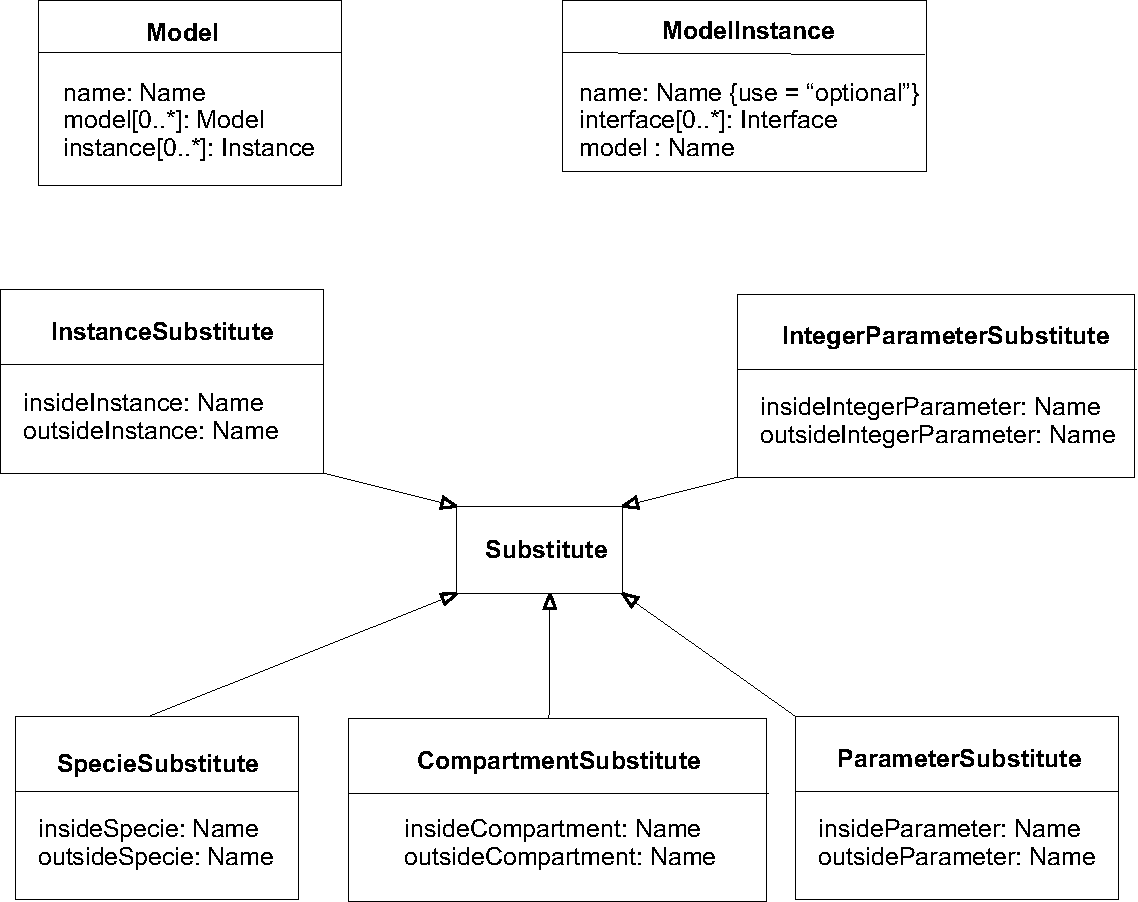
\includegraphics[scale = 0.75]{submodels}

  \caption{A diagram of the submodel class system
    (The notation used in the figures in this document is described in ~\cite{Hucka:Notation}).}

  \label{fig:submodels}

\end{figure}

A model includes zero or more models (submodels).  These are just
definitions and do not imply any occurrence of components inside
the model. A model includes zero or more model instances.  These create
occurrences of the components in the referenced submodel within
the model.  An \class{modelInstance} element contains a name attribute
\attrib{model} which refers to the submodel that should be
instantiated in the model.

For example the following xml defines a submodel XX.
The model creates two model instances p and q of the submodel XX.

\begin{quote}

  \begin{small}

    \tightspacing

\begin{verbatim}

<sbml version="2">
    <model name="simpleinstances">
        <listOfModels>
             <model name="XX">
                <listOfCompartments>
                    <compartment name="x"/>
                </listOfCompartments>
                <listOfSpecies>
                    <specie name="a" compartment="x" initialAmount="1"/>
                    <specie name="b" compartment="x" initialAmount="1"/>
                    <specie name="c" compartment="x" initialAmount="1"/>
               </listOfSpecies>
               <listOfReactions>
                    <reaction name="s1">
                        <listOfReactants>
                            <specieReference specie="a"/>
                        </listOfReactants>
                        <listOfProducts>
                            <specieReference specie="b"/>
                        </listOfProducts>
                    </reaction>
                    <reaction name="s2">
                        <listOfReactants>
                            <specieReference specie="b"/>
                        </listOfReactants>
                        <listOfProducts>
                            <specieReference specie="c"/>
                        </listOfProducts>
                    </reaction>
               </listOfReactions>
            </model>
        </listOfModels>
        <listOfModelInstances>
            <modelInstance name="p" model="XX"/>
            <modelInstance name="q" model="XX"/>
        </listOfModelInstances>
    </model>
</sbml>

\end{verbatim}

    \regularspacing

  \end{small}

\end{quote}

Figure \ref{fig:simpleinstances} shows this model diagramatically.

\begin{figure}

  \centering

  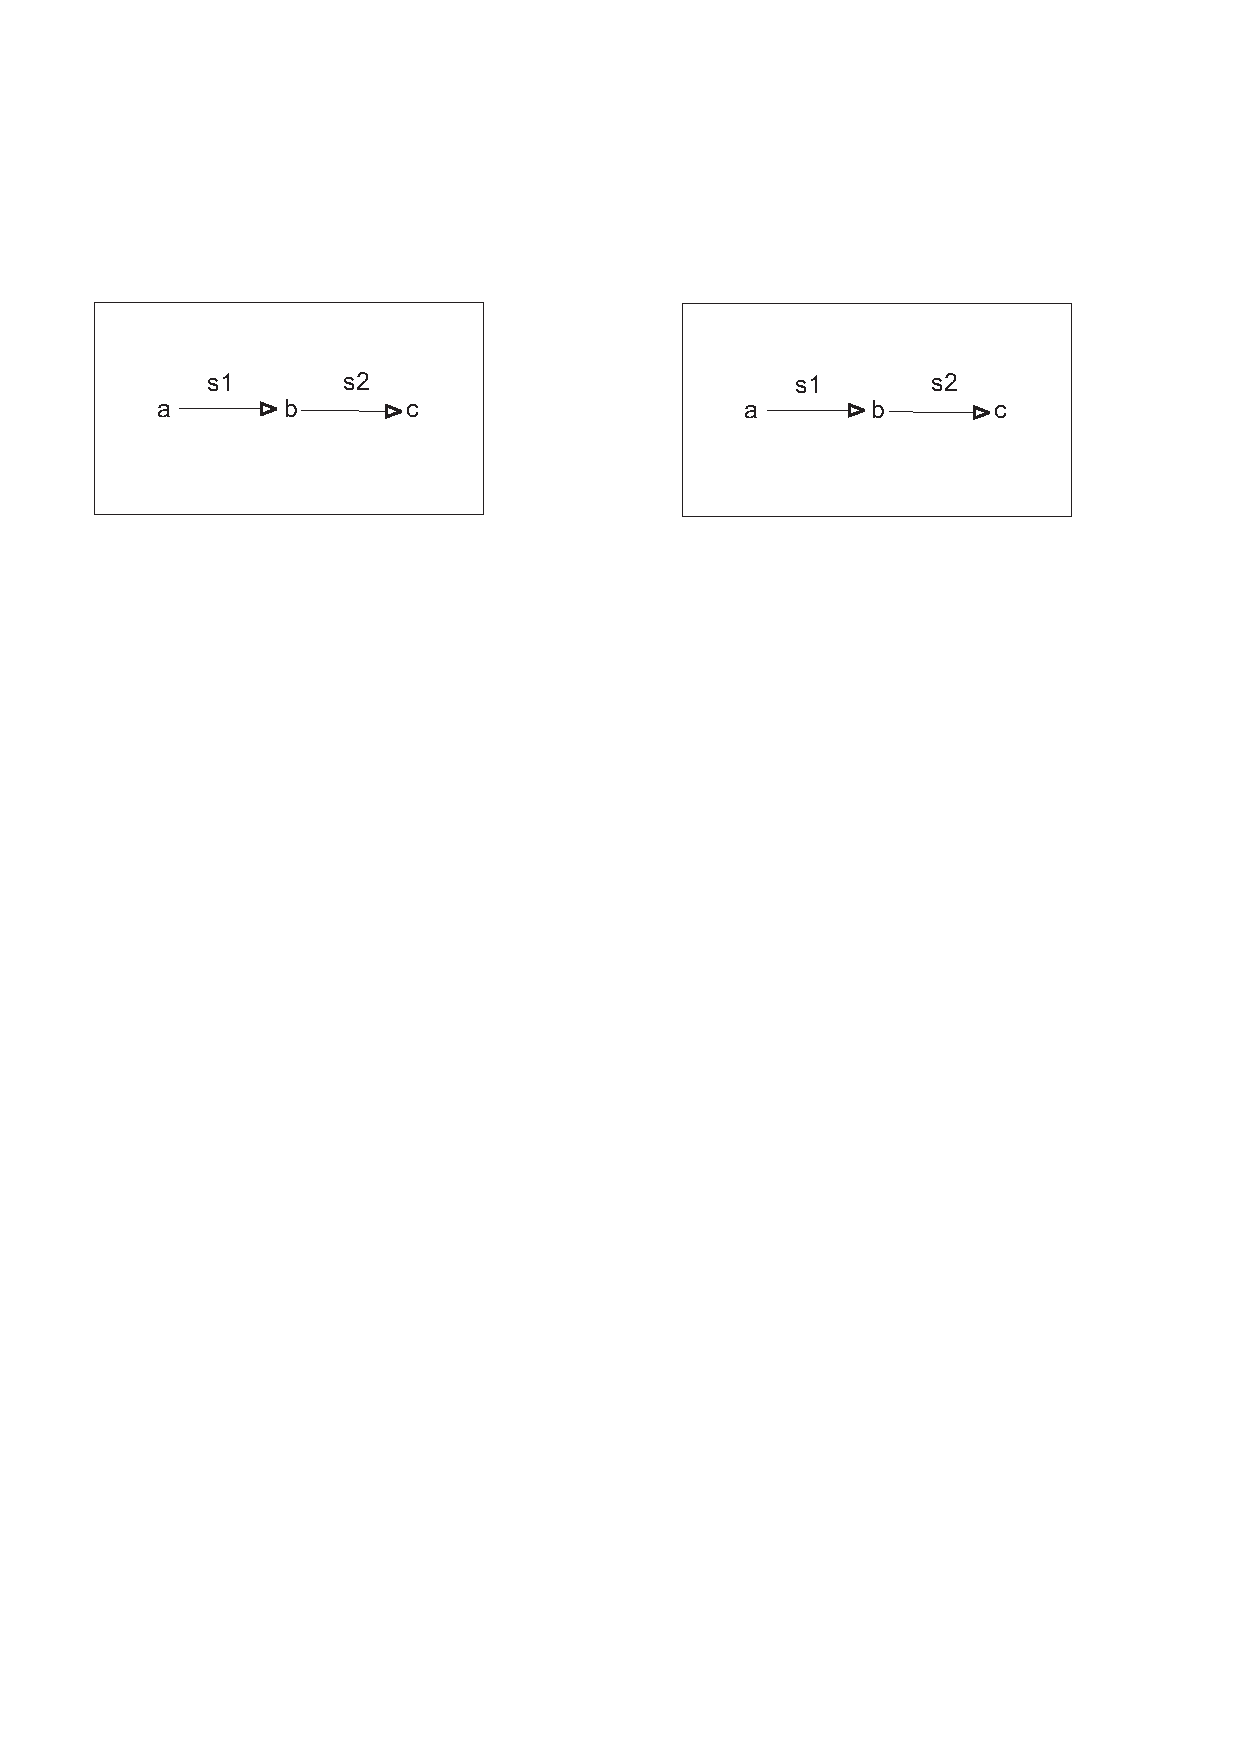
\includegraphics[scale = 0.75]{simpleinstances}

  \caption{A diagram of the simpleinstances model}

  \label{fig:simpleinstances}

\end{figure}

In this model there are now two compartments, two species and two
reactions. This is not meaningful as the species are not
connected by a reaction.

\subsection{Model Expansion and validation}
\label{sec:expansion}

This description of the submodel feature effectively defines a
transformation from a model containing submodels and model instances to
an equivalent model containing neither.  This transformation is
called \emph{expansion}.  The product of the transformation is
called the \emph{expanded} form of a model.

A model is valid if its expanded form is consistent (name
attributes refer to other named elements of the correct type) and
contains at least one compartment, one species and one reaction.
The detail of a valid expanded form will require further work.
In the meantime as a rough guide the expanded form should comply with the
current SBML definition ~\cite{Finney:SBMLv1}.

\subsection{Referencing components inside model instances}

Components inside model instances can be referenced in formulae and name
attributes by using the form \emph{instance}.\emph{component}
where \emph{component} is the name of a component inside the
model instance \emph{instance}.

For example the following fragment shows an element referring to
a species 's' inside model instance 'i'.

\begin{quote}

  \begin{small}

    \tightspacing

\begin{verbatim}

<specieReference specie="i.s"/>

\end{verbatim}

    \regularspacing

  \end{small}

\end{quote}

The following model uses this technique to create a
transport reaction between two compartments.


\begin{quote}

  \begin{small}

    \tightspacing

\begin{verbatim}

<sbml version="2">
    <model name="transport">
        <listOfModels>
             <model name="XX">
                <listOfCompartments>
                    <compartment name="inside"/>
                </listOfCompartments>
                <listOfSpecies>
                    <specie name="a" compartment="inside" initialAmount="1"/>
               </listOfSpecies>
            </model>
        </listOfModels>
        <listOfModelInstances>
            <modelInstance name="p" model="XX">
            <modelInstance name="q" model="XX">
        </listOfModelInstances>
        <listOfReactions>
            <reaction name="transport">
                <listOfReactants>
                    <specieReference specie="p.a"/>
                </listOfReactants>
                <listOfProducts>
                    <specieReference specie="q.a"/>
                </listOfProducts>
            </reaction>
        </listOfReaction>
    </model>
</sbml>

\end{verbatim}

    \regularspacing

  \end{small}

\end{quote}

Figure \ref{fig:transport} shows this model in diagram form.

\begin{figure}

  \centering

  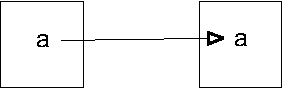
\includegraphics[scale = 0.75]{transport}

  \caption{A diagram of the transport model}

  \label{fig:transport}

\end{figure}

This notation can be used to any depth.  For example x.y.z refers
to component z inside model instance y inside model instance x. This notation
can only be used when referring to components - not declaring
them.

\subsection{Substitutes}

Individual model instances can be made unique through the use of
\class{substitute} elements, see Figure \ref{fig:submodels}. An
\class{modelInstance} element can have one or more \class{substitute}
elements.

\class{Substitute} elements define how a component in a model
('outside') can be substituted for a component 'inside' a
submodel for a given model instance. A submodel does not declare
explicitly which components can be substituted.  When a component
is substituted the values and units associated with the outside
component replace those of the inside component.

For example if we want to locate a model instance in a given
compartment rather than the compartment that it was originally
defined in by its submodel definition we can substitute another
compartment for the original compartment as part of the
\class{modelInstance} element.  The original compartment is 'inside'
the model instance and the substitute compartment is 'outside'.

This mechanism allows model instances to share common components by
allowing a single component to be substituted into more than one
model instance.

There are several different subtypes of \class{Substitute} one for
each type of component, see Figure \ref{fig:submodels}.  All
these types have a similar form. These types have a name
attribute of the form \attrib{insideX} which refers to a
component of the respective type inside the model instance. The
\class{substitute} elements have an attribute of the form
\attrib{outsideX} which refers to a component in the model (as
opposed to the submodel).

\subsection{Missing attributes}

It is not necessary for components inside a submodel to have a
complete set of attribute values. In a model's expanded form
these attributes should have acquired values through the use of
\class{substitute} elements.  For example all specie elements which don't
have values for their \attrib{initialAmount} can only occur
inside submodels.  Instances of these submodels must have
\class{substitute} elements which substitute species which do have values
for their \attrib{initalAmount} attributes.

Table \ref{tab:attributes} lists the attributes that are optional
in the unexpanded form of SBML. These attributes have to be either
resolved in the expanded form through substitution or defaulted.

\begin{table}[tb]
\begin{tabular}{lll}

  \textbf{Element} & \textbf{Attribute} & \textbf{Resolved Constraint} \\

  \hline

  specie & compartment & use="required"\\
  specie & initialAmount & use="required"\\
  specie & boundaryCondition & use="default" value="false" \\
  parameter & value & use="required"\\
  integerParameter & value & eliminated by expansion\\
  compartment & volume & use="default" value="1" \\
  modelInstance & model & eliminated by expansion\\
\end{tabular}

\caption{Attributes that become optional in this proposed
version.  The constraint column shows the constraint on
the attribute in the expanded form.}

\label{tab:attributes}
\end{table}

The above example model "simpleinstances" can be modified allowing the two
model instances to form a pathway as follows.
\begin{quote}

  \begin{small}

    \tightspacing

\begin{verbatim}

<sbml version="2">
    <model name="connectedinstances">
        <listOfModels>
             <model name="XX">
                <listOfCompartments>
                    <compartment name="inside"/>
                </listOfCompartments>
                <listOfSpecies>
                    <specie name="a"/>
                    <specie name="b" compartment="inside" initialAmount="1"/>
                    <specie name="c"/>
               </listOfSpecies>
               <listOfReactions>
                    <reaction name="s1">
                        <listOfReactants>
                            <specieReference specie="a"/>
                        </listOfReactants>
                        <listOfProducts>
                            <specieReference specie="b"/>
                        </listOfProducts>
                    </reaction>
                    <reaction name="s2">
                        <listOfReactants>
                            <specieReference specie="b"/>
                        </listOfReactants>
                        <listOfProducts>
                            <specieReference specie="c"/>
                        </listOfProducts>
                    </reaction>
               </listOfReactions>
            </model>
        </listOfModels>
        <listOfCompartments>
            <compartment name="outside"/>
        </listOfCompartments>
        <listOfSpecies>
            <specie name="aa" compartment="x" initialAmount="1"/>
            <specie name="ca" compartment="x" initialAmount="1"/>
            <specie name="cc" compartment="x" initialAmount="1"/>
        </listOfSpecies>
        <listOfModelInstances>
            <modelInstance name="p" model="XX">
                <listOfSubstitutes>
                    <speciesSubstitute insideSpecie="a" outsideSpecie="aa"/>
                    <speciesSubstitute insideSpecie="c" outsideSpecie="ca"/>
                </listOfSubstitutes>
            </modelInstance>
            <modelInstance name="q" model="XX"/>
                <listOfSubstitutes>
                    <speciesSubstitute insideSpecie="a" outsideSpecie="ca"/>
                    <speciesSubstitute insideSpecie="c" outsideSpecie="cc"/>
                </listOfSubstitutes>
            </modelInstance>
        </listOfModelInstances>
    </model>
</sbml>

\end{verbatim}

    \regularspacing

  \end{small}

\end{quote}

Figure \ref{fig:connectedinstances} shows this model in diagram form.

\begin{figure}

  \centering

  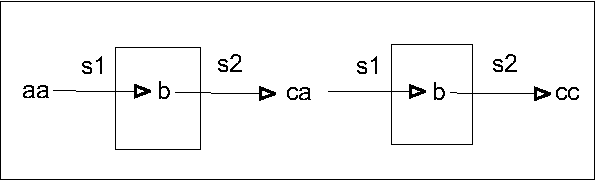
\includegraphics[scale = 0.75]{connectedinstances}

  \caption{A diagram of the connectedinstances model}

  \label{fig:connectedinstances}

\end{figure}

\subsection{Missing components}

A model can have zero or more of any compartments, species,
model instances or reactions. The expanded form of a model should
consist of at least one compartment, specie and reaction.

\subsection{Units}
[Ed - this section will be extended with examples in the future]

\subsubsection{Built-in Units}
A submodel can use different unit scales for component values of
built-in units, eg volume, from those used by a model containing
an instance of the submodel. When an \class{modelInstance} element has
\class{substitute} elements which substitute components containing
values at a different scales to the replaced components, the
values from the substituted component are implicitly scaled to
the scale used in the submodel.

\subsubsection{Parameter Units}
A similar scheme is used for \class{Parameter} elements.  As for
built-in types the scale of a substituted parameter value can be
different from the scale of the replaced parameter.  This assumes
that the \class{Unit} of the two \class{Parameter} elements are
equivalent [Ed - this needs careful definition].

In fact substituted \class{Parameter} elements must always have
\class{Unit} elements equivalent to the \class{Parameter}
elements that are replaced. This is a form of type checking.
A \class{Parameter} element in a submodel which has no
\class{Unit} can be replaced by any \class{Parameter} element
through substitution.  The opposite is not true.

\section{Arrays of Components}

It has become apparent that many systems biology simulations
require arrays of components. The following section describes a
scheme to support this.

The following components can occur in arrays: model instances,
compartments, geometry, mapping, species, parameters, rules and
reactions. Each of these elements can contain a list of
\class{dimension} elements, see Figure \ref{fig:dimension}. This
diagram shows the \class{NeighborhoodDimension} class which is
detailed in the next section.

A dimension element has a \attrib{name} name attribute and two
integer expression attributes \attrib{start} and
\attrib{finish} which define the range of the array in that
dimension.

The name attribute declares the given name as a symbol that can
be used in integer expressions.

\begin{figure}

  \centering

  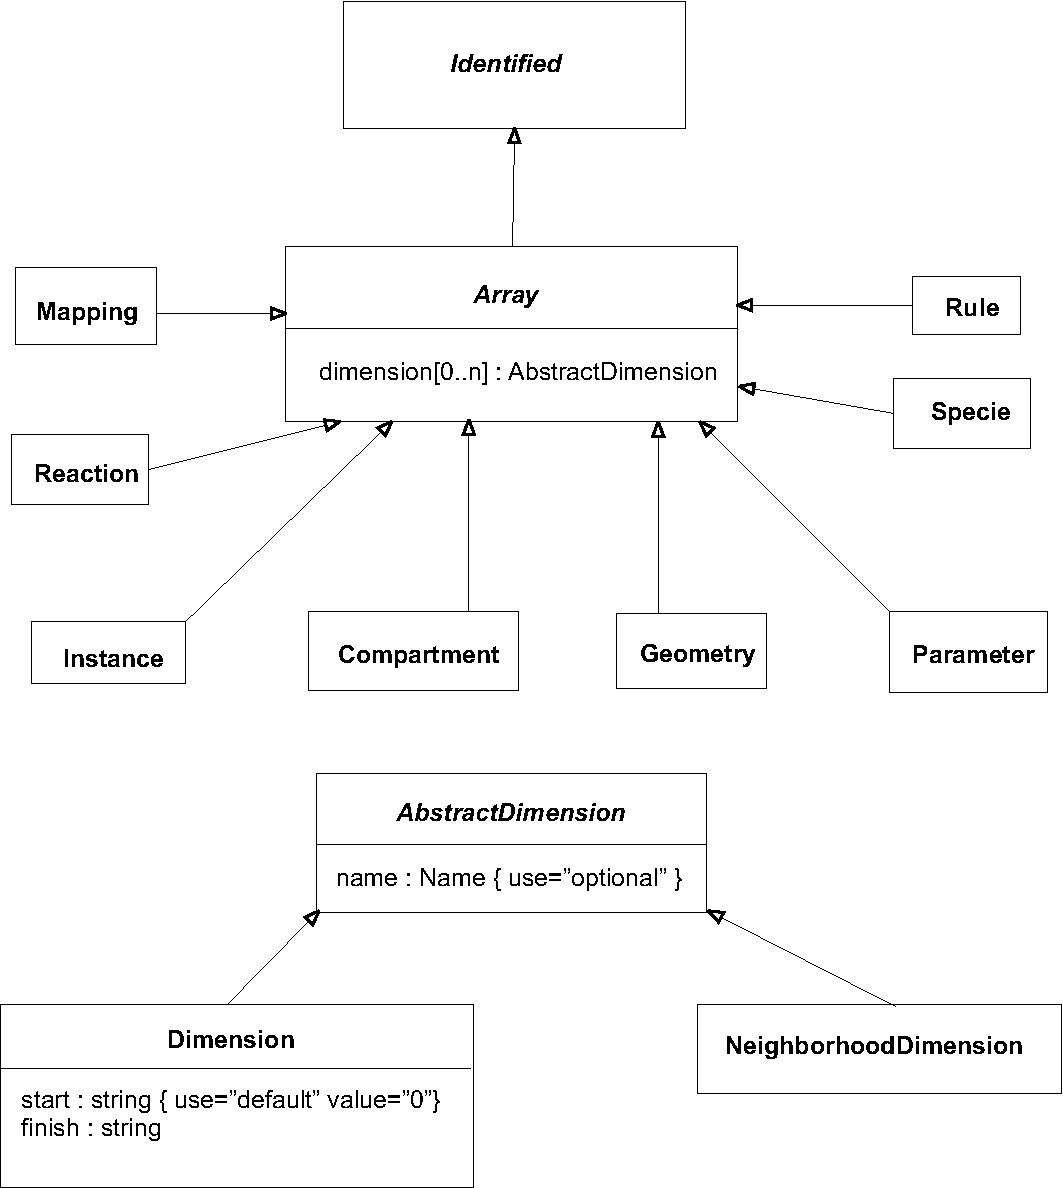
\includegraphics[scale = 0.75]{dimension}

  \caption{The Dimension class}

  \label{fig:dimension}

\end{figure}

For example here's a two dimensional array of compartments:

\begin{quote}
  \begin{small}
    \tightspacing

\begin{verbatim}

<compartment name="cell" volumne="1">
    <listOfDimensions>
        <dimension name="x" start="0" finish="9"/>
        <dimension name="y" start="0" finish="9"/>
    </listofDimensions>
</compartment>

\end{verbatim}

    \regularspacing
  \end{small}
\end{quote}

\subsection{Expansion and validity}

The principle of expansion defined in section \ref{sec:expansion} applies to
arrays.  The expanded form of a model doesn't contain any \class{dimension} elements.
There is no difference in the validity of the expanded form of models containing
arrays or submodels.

\subsection{Refering to array elements}

Names can be followed by an array element postfix operator \verb+[]+ where the brackets contain a comma
separated sequence of integer expressions. The number of integer
expressions should be the number of dimensions of the element
declaring the symbol. This notation can only be used in name
fields and symbols in formulae refering to components.

For example here's a species placed inside
an element of the previous array of compartments.

\begin{quote}
  \begin{small}
    \tightspacing

\begin{verbatim}

<specie name="s" initialAmount="1" compartment="cell[0,0]"/>
\end{verbatim}

    \regularspacing
  \end{small}
\end{quote}

As another example here's an array of species placed inside the
previous array of compartments.

\begin{quote}
  \begin{small}
    \tightspacing

\begin{verbatim}

<specie name="s" initialAmount="1" compartment="cell[xd,yd]">
    <listOfDimensions>
        <dimension name="xd" start="0" finish="9"/>
        <dimension name="yd" start="0" finish="9"/>
    </listofDimensions>
</specie>

\end{verbatim}

    \regularspacing
  \end{small}
\end{quote}

For example here's a rule applied to a species array.

\begin{quote}
  \begin{small}
    \tightspacing

\begin{verbatim}

<listOfSpecies>
    <specie name="s" initialAmount="1" compartment="cell">
        <listOfDimensions>
            <dimension name="i" start="0" finish="9"/>
        </listOfDimensions>
    </specie>
</listOfSpecies>
<listOfRules>
    <specieRule specie="z" formula="t-s[i]"/>
        <listOfDimensions>
            <dimension name="i" start="0" finish="9"/>
        </listOfDimensions>
    </specieRule>
</listOfRules>

\end{verbatim}

    \regularspacing
  \end{small}
\end{quote}

This notation for referring to components inside array can be
combined with the model instance component reference notation. For example accessing a specie inside a array of model instances:

\begin{quote}
  \begin{small}
    \tightspacing

\begin{verbatim}

<listOfModels>
    <model name="submodel">
        <listOfSpecies>
            <specie name="s" initialAmount="1" compartment="cell"/>
        </listOfSpecies>
    </model>
</listOfModels>
<listOfModelInstances>
    <modelInstance name="I" model="submodel">
        <listOfDimensions>
            <dimension name="i" start="0" finish="9"/>
        </listOfDimensions>
    </modelInstance>
</listOfModelInstances>
<listOfRules>
    <specieRule specie="z" formula="t-I[i].s"/>
        <listOfDimensions>
            <dimension name="i" start="0" finish="9"/>
        </listOfDimensions>
    </specieRule>
</listOfRules>

\end{verbatim}

    \regularspacing
  \end{small}
\end{quote}

The opposite access method is possible as well, accessing a array of species inside a model instance:

\begin{quote}
  \begin{small}
    \tightspacing

\begin{verbatim}

<listOfModels>
    <model name="submodel">
        <listOfSpecies>
            <specie name="s" initialAmount="1" compartment="cell">
                <listOfDimensions>
                    <dimension name="i" start="0" finish="9"/>
                </listOfDimensions>
            </specie>
        </listOfSpecies>
    </model>
</listOfModels>
<listOfModelInstances>
    <modelInstance name="I" model="submodel"/>
</listOfModelInstances>
<listOfRules>
    <specieRule specie="z" formula="t-I.s[i]"/>
        <listOfDimensions>
            <dimension name="i" start="0" finish="9"/>
        </listOfDimensions>
    </specieRule>
</listOfRules>

\end{verbatim}

    \regularspacing
  \end{small}
\end{quote}

\section{Neighborhoods}

To further improve the modeling of arrays of biological entities
we propose the concept of neighborhoods.  A \class{neighborhood}
is a mapping from an integer co-ordinate, \emph{source}, to
a set of integer co-ordinates, \emph{connections}.  A
\class{neighborhood} can be defined for any number of dimensions.

The structure of \class{neighborhood} is shown in figure
\ref{fig:neighborhood}.  A \class{neighborhood} element contains
a number of \class{dimension} elements that define the range of
possible connections in each dimension.  These elements do not
define the set of all connections but just restrict the possible
connections to this range.  The name attribute on
\class{dimension} elements inside a \class{neighborhood} is
redundant.

\begin{figure}

  \centering

  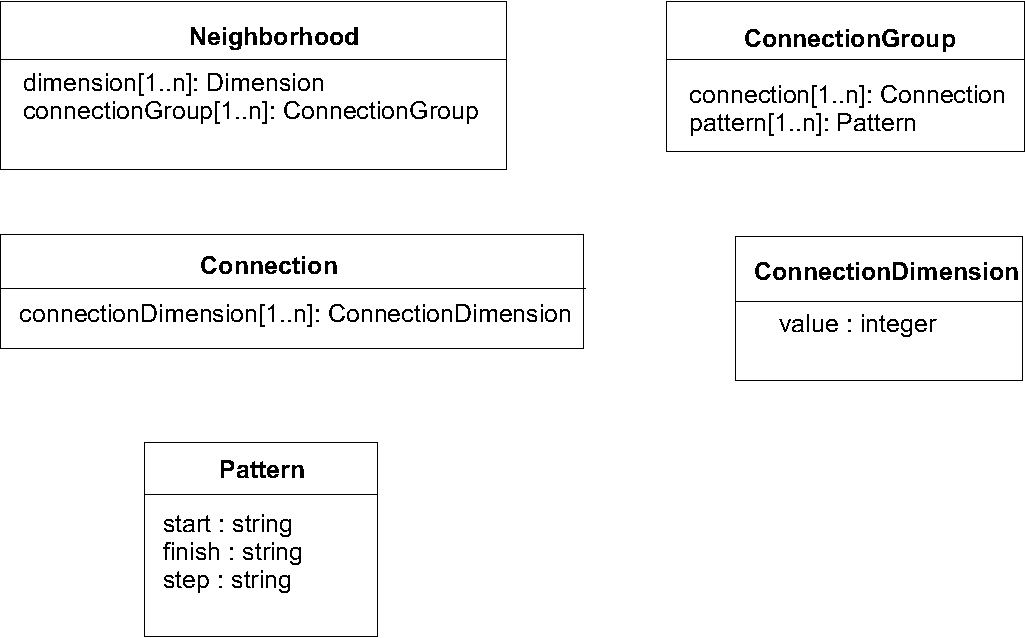
\includegraphics[scale = 0.75]{neighborhood}

  \caption{\class{Neighborhood} and related classes}

  \label{fig:neighborhood}

\end{figure}

A \class{neighborhood} is defined by a set of
\class{connectionGroup} elements.  A \class{connectionGroup}
consists of a set of \class{connection} elements. A
\class{connection} element is a co-ordinate relative to a source
 and is comprised of a list of \class{connectionDimension}
elements, one for each \class{dimension} of the
\class{neighborhood}.

A \class{connectionGroup} has a \class{pattern} element for each
dimension that describes which source co-ordinates the
\class{connectionGroup} is applied to.  The \class{pattern}
string - integer formula - attributes \attrib{start},
\attrib{finish} and \attrib{step} define a loop.  Each iteration
of the loop defines a location where the \class{connectionGroup}
source occurs.

The set of unbounded connections at a given location is the union
of the set of \class{connection} elements of those
\class{connectionGroup} elements that have a source that occurs
at that location. The source co-ordinate is added to the given
connection co-ordinate.  The actual set of connections at a
source is the intersection of the unbounded connections with the
range defined by the \class{dimension} elements enclosed in the
\class{neighborhood} element.

Each \class{pattern} and \class{connectionDimension} element
corresponds to one dimension of the co-ordinate system that the
\class{neighborhood} can be applied to. All lists containing
\class{dimension}, \class{pattern} and
\class{connectionDimension} elements should have the same number
of elements when enclosed in the same neighborhood element

A \class{neighborhood} consists of several
\class{connectionGroup} elements so that its possible to define
hexagonal connections in a 2D grid.

For example here's a simple 1 dimensional neighborhood:
\begin{quote}
  \begin{small}
    \tightspacing

\begin{verbatim}

<neighborhood name="one_d">
    <listOfDimensions>
        <dimension start="0" finish="8">
    </listOfDimensions>
    <listOfConnectionGroups>
        <connectionGroup>
            <listOfPatterns>
                <pattern start="0" finish="8" step="1"/>
            </listOfPatterns>
            <listOfConnections>
                <connection>
                    <listOfConnectionDimensions>
                        <connectionDimension value="1"/>
                    </listOfConnectionDimensions>
                </connection>
            </listOfConnections>
        </connectionGroup>
    </listOfConnectionGroups>
</neighborhood>

\end{verbatim}

    \regularspacing
  \end{small}
\end{quote}

In the example given a co-ordinate of x in the range 0 to 8 is
mapped to the set consisting of one integer x + 1. Any value
outside that range results in an empty set.  Obviously this
example doesn't amount to much however it is possible to create
hexagon patterns using this scheme see appendix \ref{sec:completeexample}.

[Ed - Add description of algorithm for mapping a given co-ordinate to a
the set of co-ordinates that is the set of connections for the
given co-ordinate]

\subsection{Using neighborhoods for creating arrays}

A neighborhood can be referenced as a way to create an array that
has a variable number of elements in one dimension. The number of
elements at given co-ordinate is the the number of connections
present in neighborhood at that location.  This is achieved by
using a \class{neighborhoodDimension} element, see figure
\ref{fig:neighborhoodDimension}, as a dimension in place of a
\class{dimension} element.  Like a \class{dimension} element a
\class{neighborhoodDimension} element has a name attribute which
declares a integer symbol.

\begin{figure}

  \centering

  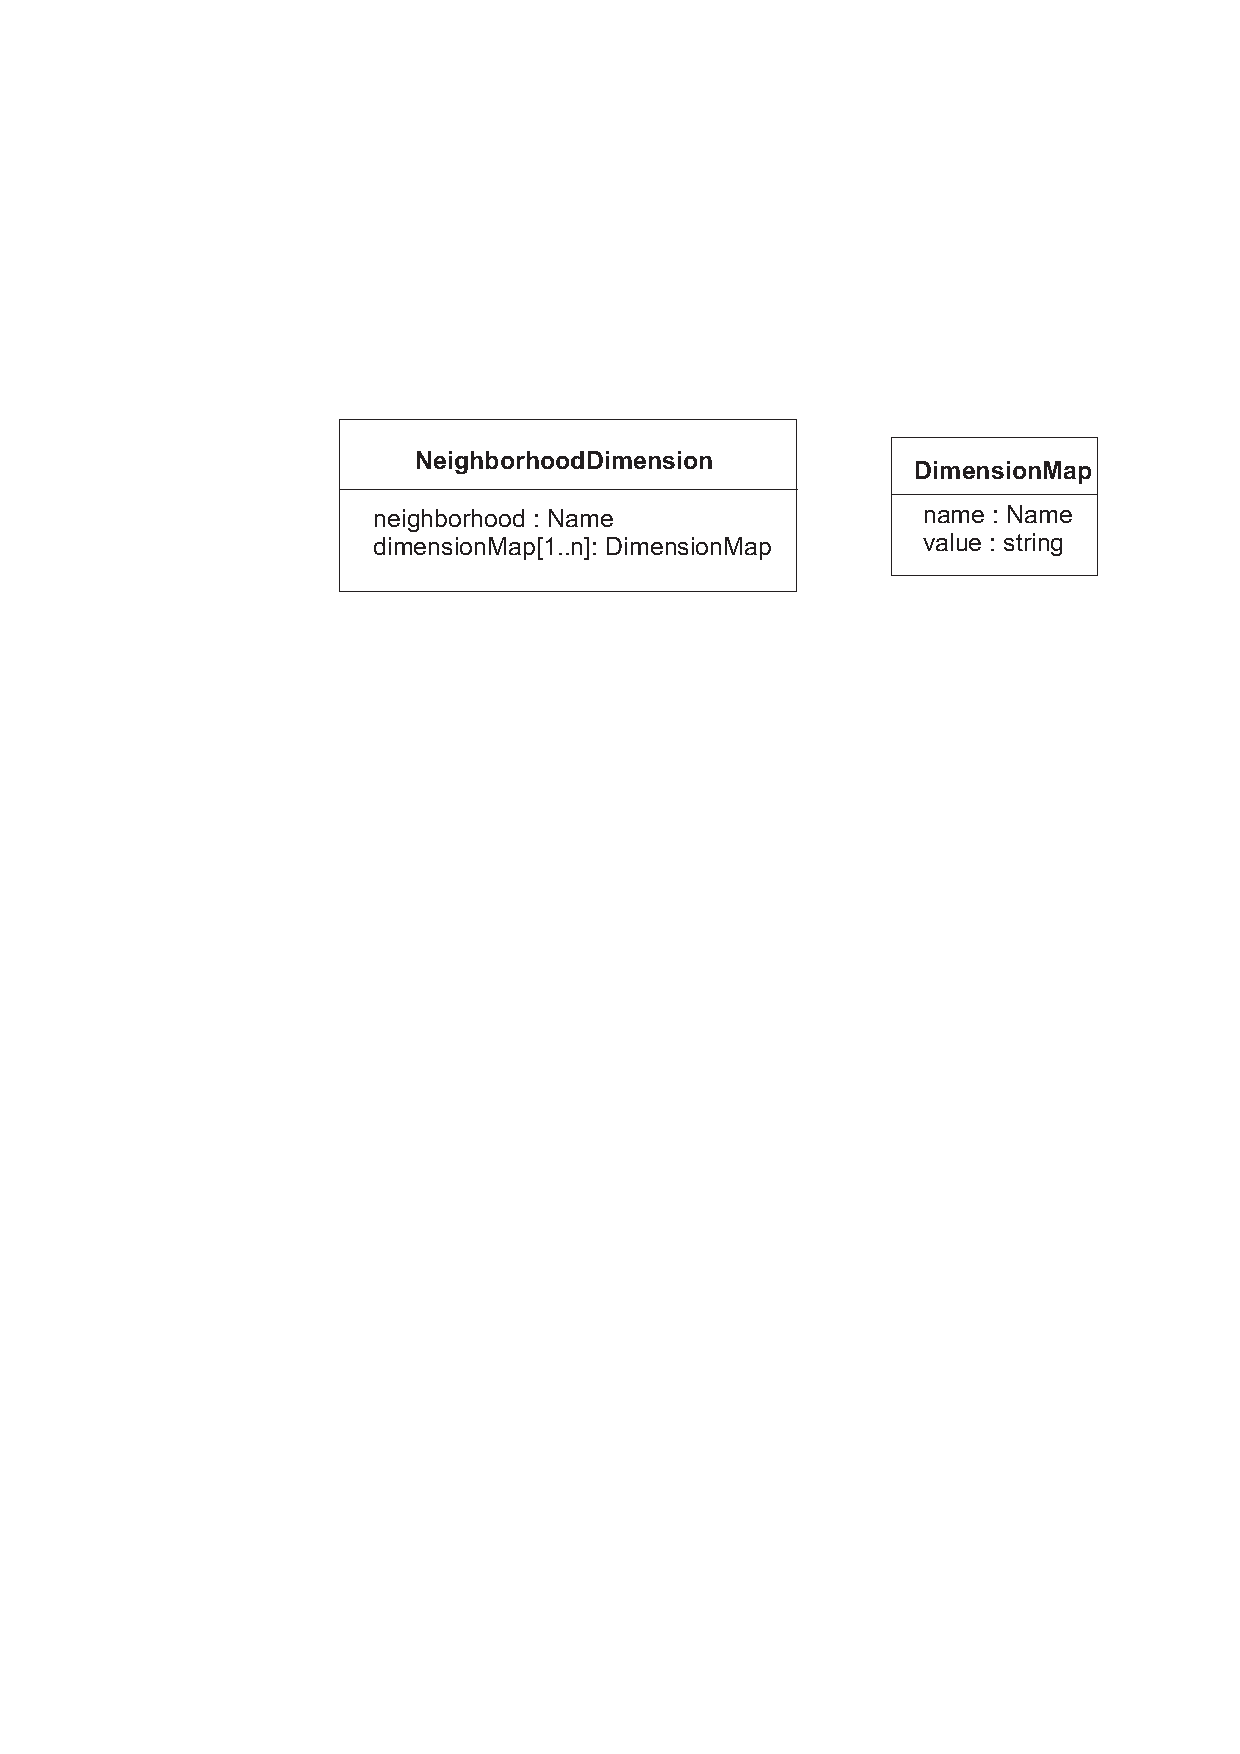
\includegraphics[scale = 0.75]{neighborhoodDimension}

  \caption{\class{NeighborhoodDimension} and related classes}

  \label{fig:neighborhoodDimension}

\end{figure}

A \class{neighborhoodDimension} element contains a list of
dimensionMap elements.  Each \class{dimensionMap} instantiates
one integer symbol through its name attribute and supplies the
value for the source co-ordinate in the corresponding dimension
through its value attribute which is an integer expression.

For example here's an array of reactions for each connection in
the previous xml fragment:

\begin{quote}
  \begin{small}
    \tightspacing
\begin{verbatim}
<listOfSpecies>
    <specie name="s" initialAmount="1" compartment="cell[i]">
        <listOfDimensions>
            <dimension name="i" start="0" finish="9"/>
        </listOfDimensions>
    </specie>
</listOfSpecies>
....
<reaction name="transport" reversible="true">
    <listOfDimensions>
        <dimension name="i" start="0" finish="9"/>
        <neighborhoodDimension name="j" neighborhood="one-d">
            <dimensionMap name="k" value="i"/>
        </neighborhoodDimension>
    </listOfDimensions>
    <listOfProducts>
        <speciesReference specie="s[i]"/>
    </listOfProducts>
    <listOfReactant>
        <speciesReference specie="s[k]"/>
    </listOfReactants>
</reaction>

\end{verbatim}
    \regularspacing
  \end{small}
\end{quote}

\section{Math for arrays and neighborhoods}

\subsection{Matrix functions}

Matrix functions can appear in float formulas.  A scheme for product and sum functions is described here but other types of matrix functions
are probably possible with further thought.

The sequence of the arguments to these functions are of the form
$ integerDeclaration_{0}, \ldots, integerDeclaration_{n}, f$ where
\begin{itemize}
\item $ integerDeclaration_{i} $ := $ simpleDeclaration_{i} | mappedDeclaration_{i} $
\item $f$ is a float expression that can contain integer symbols declared in $simpleDeclaration$ and $mappedDeclaration$
\item $ simpleDeclaration_{i} $ is $i_{i}, is_{i}, if_{i}$
\item $i_{i}$ is a new integer symbol,
\item $is_{i}$ and $if_{i}$ are integer expressions which define the
range of $i_{i}$
\item $ mappedDeclaration_{i} $ is $ neighborhood $ $ neighborhoodname [j_{i}], k_{i,0}, l_{i,0}
\ldots, k_{i,m}, l_{i,m} $
\item $neighborhood$ is literal
\item $neighborhoodname$ is the name of a \class{neighborhood} element
\item $j_{i}$ is an new integer symbol which runs over a set of connections in the given neighborhood,
\item $k_{i,h}$ is a new integer symbol mapped by the given neighborhood
\item $l_{i,h}$ is an integer expression which is the input co-ordinate to the neighborhood
\end{itemize}
There is a pair of $k_{i,h}$ and $l_{i,h}$ for each
\class{dimension} in the \class{neighborhood} refereed to by the
preceding $neighborhoodname$

For example consider a reaction affected by product of the concentrations of a set of species:

\begin{quote}
  \begin{small}
    \tightspacing
\begin{verbatim}

<listOfSpecies>
    <specie name="s" initialAmount="1" compartment="cell"/>
    <specie name="p" initialAmount="0" compartment="cell"/>
    <specie name="c" initialAmount="1" compartment="cell">
        <listOfDimensions>
            <dimension name="i" start="0" finish="9"/>
        </listOfDimensions>
    </specie>
</listOfSpecies>
....
<reaction name="complex" reversible="true">
    <listOfProducts>
        <speciesReference specie="p"/>
    </listOfProducts>
    <kineticLaw formula="k * product(i, 0, 9, c[i])">
        <listOfParameters>
            <parameter name="k" value="0.25"/>
        </listOfParameter>
    </kineticLaw>
    <listOfReactant>
        <speciesReference specie="s"/>
    </listOfReactants>
</reaction>

\end{verbatim}
    \regularspacing
  \end{small}
\end{quote}

As another example we add a similar reaction to the previous example using neighborhoods:

\begin{quote}
  \begin{small}
    \tightspacing
\begin{verbatim}
<listOfSpecies>
    <specie name="s" initialAmount="1" compartment="cell">
        <listOfDimensions>
            <dimension name="i" start="0" finish="9"/>
        </listOfDimensions>
    </specie>
    <specie name="p" initialAmount="1" compartment="cell">
        <listOfDimensions>
            <dimension name="i" start="0" finish="9"/>
        </listOfDimensions>
    </specie>
</listOfSpecies>
....
<reaction name="z" reversible="true">
    <listOfDimensions>
        <dimension name="i" start="0" finish="9"/>
    </listOfDimensions>
    <listOfProducts>
        <speciesReference specie="s[i]"/>
    </listOfProducts>
    <kineticLaw formula="product(neighborhood one-d, i, connection, s[connection])"/>
    <listOfReactant>
        <speciesReference specie="p[i]"/>
    </listOfReactants>
</reaction>

\end{verbatim}
    \regularspacing
  \end{small}
\end{quote}

\subsection{Integer Parameters}

A model can have a list of integer parameters.
%see figure \ref{fig:integerConstant}.
An \class{integerParameter} element has a name attribute and an
integer \attrib{value} attribute. The name values on these
elements can be used as symbols in integer expressions in which
case the value of \attrib{value} attribute is substituted.  An
expanded form of model must not contain \class{integerParameter}
elements.

\subsection{Integer Expressions}

Integer expressions occur in various places in the above scheme.
Integer expressions are similar to float expressions except that
only $+$, $-$, $*$ and $/$ operations are available and the
symbols are the names of either \class{dimension} or
 elements associated with the formula, the name of
\class{integerParameter} elements or declared by an sum or product
function call.

%=============================================================================
\setcounter{secnumdepth}{-1}
\section{Appendix}
\setcounter{secnumdepth}{2}
\appendix

%=============================================================================

\section{A complete model using model instances and arrays}

\label{sec:completeexample}

This model is comprised of 10000 'cells' arranged in 2 dimensions
as a square 100 cells on a side. The cells are connected to six
nearest neighbors to simulate a hexagonal tessalation of the
cells.

\subsection{Creating a neighborhood for a hexagonal tessalation}

The method for creating a neighborhood which simulates a
hexagonal tessalation is shown in figure \ref{fig:hexagon}.  For
this figure you can see that this requires 2 sets of connections:
one for even columns and the other for odd columns.  This is
represented in the SBML model as two \class{connectionGroup}
elements.

\begin{figure}

  \centering

  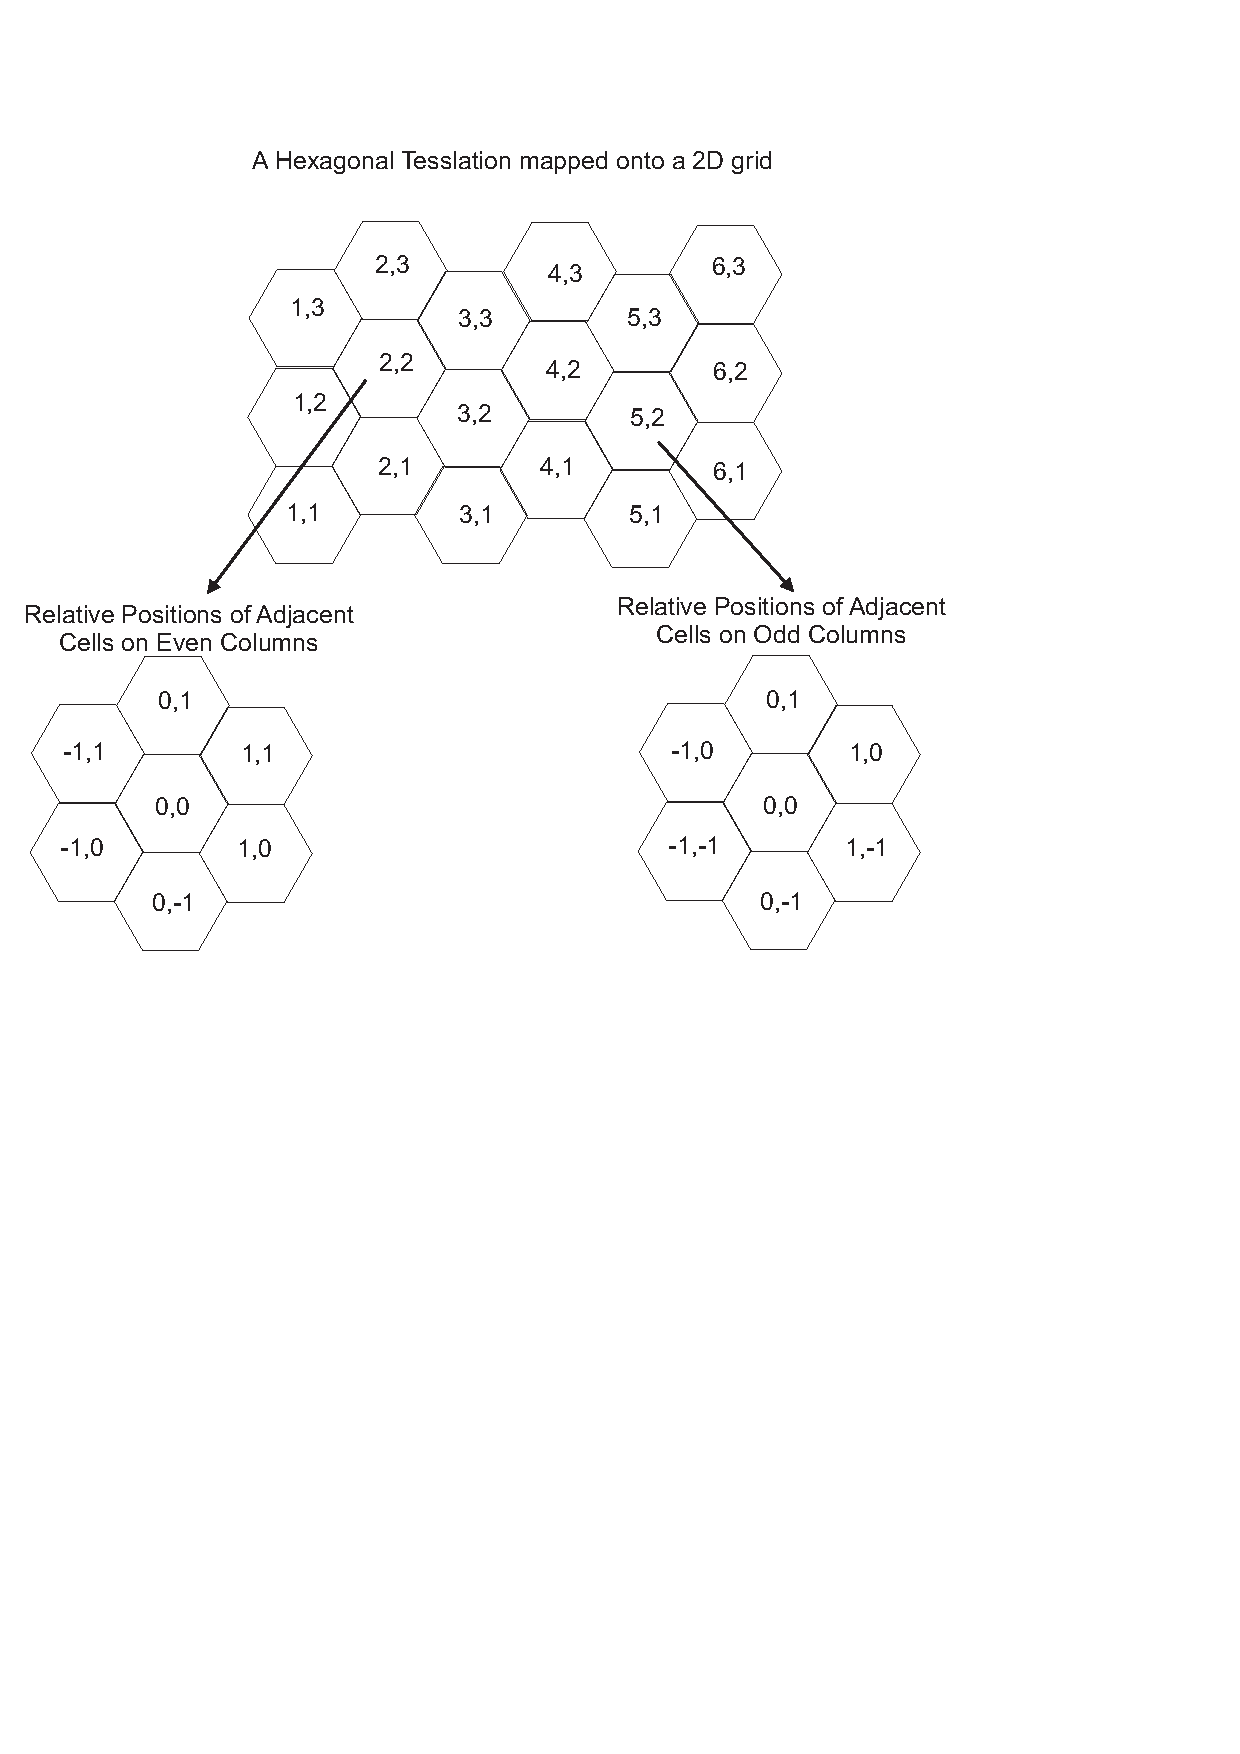
\includegraphics[scale = 0.75]{hexagon}

  \caption{Mapping a hexagonal connection scheme onto connections in a 2D array}

  \label{fig:hexagon}

\end{figure}

\subsection{Reactions}

The reactions in this model are shown figure \ref{fig:cell}.
The model is not biologically meaningful.  The duplicate reactions in the
adjacent cell are not shown.  None of the reactions are reversible.

\begin{figure}

  \centering

  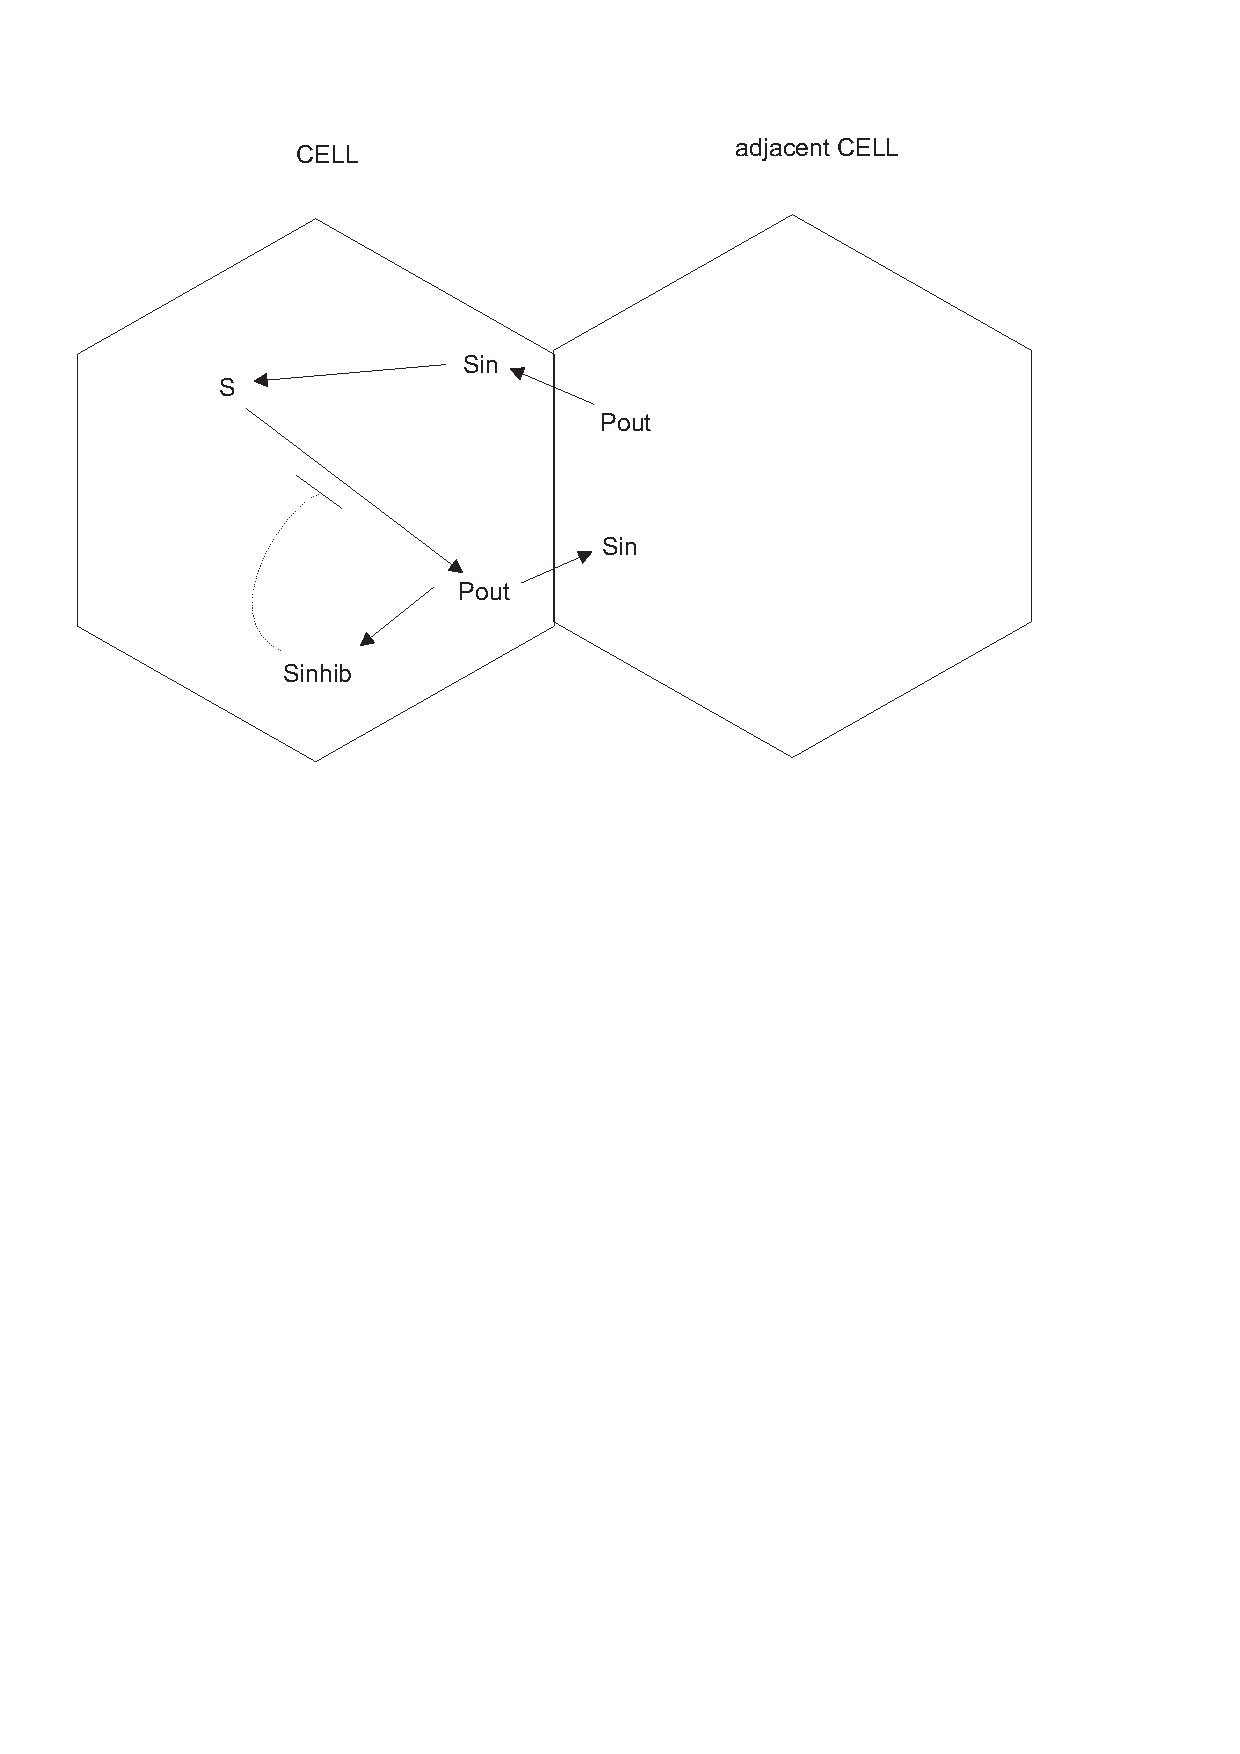
\includegraphics[scale = 0.75]{cell}

  \caption{The reaction pathway modeled in the SIMPLE\_HEXAGON model}

  \label{fig:cell}

\end{figure}

\subsection{The Model in XML}

\begin{quote}
  \begin{small}
    \tightspacing
\begin{verbatim}

<sbml version="2">

    <model name="SIMPLE_HEXAGON">
        <listOfModels>

            <model name="CELL">

                <listOfCompartments>
                    <compartment name="cell">
                </listOfCompartments>

                <listOfSpecies>
                    <specie name="Sin" compartment="cell" initialAmount="1"/>
                    <specie name="S" compartment="cell" initialAmount="0"/>
                    <specie name="Sinhib" compartment="cell" initialAmount="0"/>
                    <specie name="Pout" compartment="cell" initialAmount="0"/>
                </listOfSpecie

                <listOfReactions>

                    <reaction name="J1">
                        <listOfReactants>
                            <speciesReference name="Sin">
                        </listOfReactants>
                        <listOfProducts>
                            <speciesReference name="S">
                        </listOfProducts>
                        <kinecticLaw formula="uui(Sin, Vm, Km)"/>
                        <listOfParameters>
                            <parameter name="Vm" value="1"/>
                            <parameter name="Km" value="1"/>
                        </listOfParameters>
                    </reaction>

                    <reaction name="J2">
                        <listOfReactants>
                            <speciesReference name="S">
                        </listOfReactants>
                        <listOfProducts>
                            <speciesReference name="Pout">
                        </listOfProducts>
                        <kinecticLaw formula="unii(S, Sinhib, V, Ki)"/>
                        <listOfParameters>
                            <parameter name="V" value="1"/>
                            <parameter name="Km" value="1"/>
                            <parameter name="Ki" value="1"/>
                       </listOfParameters>
                    </reaction>

                    <reaction name="J3">
                        <listOfReactants>
                            <speciesReference name="Pout">
                        </listOfReactants>
                        <listOfProducts>
                            <speciesReference name="Sinhib">
                        </listOfProducts>
                        <kinecticLaw formula="uui(S, Vm, Km)"/>
                        <listOfParameters>
                            <parameter name="Vm" value="1"/>
                            <parameter name="Km" value="1"/>
                       </listOfParameters>
                    </reaction>

                </listOfReactions>
            </model>
        </listOfModels>

        <listOfIntegerConstants>
            <integerConstant name="size" value="100" />
        <listOfIntegerConstants>

        <listOfNeighborhoods>
            <neighborhood name="hexagon">
                <listOfDimensions>
                    <dimension start="1" finish="size"/>
                    <dimension start="1" finish="size"/>
                </listOfDimensions>
                <listOfConnectionGroups>
                    <connectionGroup name="odd_columns">
                        <listOfPatterns>
                            <pattern start="1" finish="size" step="2"/>
                            <pattern start="1" finish="size" step="1"/>
                        </listOfPatterns>
                        <listOfConnections>
                            <connection>
                                <listOfConnectionDimensions>
                                    <connectionDimension value="0">
                                    <connectionDimension value="1">
                                </listOfConnectionDimensions>
                            </connection>
                             <connection>
                                <listOfConnectionDimensions>
                                    <connectionDimension value="1">
                                    <connectionDimension value="1">
                                </listOfConnectionDimensions>
                            </connection>
                            <connection>
                                <listOfConnectionDimensions>
                                    <connectionDimension value="1">
                                    <connectionDimension value="0">
                                </listOfConnectionDimensions>
                            </connection>
                            <connection>
                                <listOfConnectionDimensions>
                                    <connectionDimension value="0">
                                    <connectionDimension value="-1">
                                </listOfConnectionDimensions>
                            </connection>
                            <connection>
                                <listOfConnectionDimensions>
                                    <connectionDimension value="-1">
                                    <connectionDimension value="0">
                                </listOfConnectionDimensions>
                            </connection>
                            <connection>
                                <listOfConnectionDimensions>
                                    <connectionDimension value="-1">
                                    <connectionDimension value="1">
                                </listOfConnectionDimensions>
                            </connection>
                       </listOfConnections>
                    </connectionGroup>
                    <connectionGroup name="even_columns">
                        <listOfPatterns>
                            <pattern start="0" finish="size" step="2"/>
                            <pattern start="2" finish="size" step="1"/>
                        </listOfPatterns>
                        <listOfConnections>
                            <connection>
                                <listOfConnectionDimensions>
                                    <connectionDimension value="0">
                                    <connectionDimension value="1">
                                </listOfConnectionDimensions>
                            </connection>
                             <connection>
                                <listOfConnectionDimensions>
                                    <connectionDimension value="1">
                                    <connectionDimension value="1">
                                </listOfConnectionDimensions>
                            </connection>
                            <connection>
                                <listOfConnectionDimensions>
                                    <connectionDimension value="1">
                                    <connectionDimension value="0">
                                </listOfConnectionDimensions>
                            </connection>
                            <connection>
                                <listOfConnectionDimensions>
                                    <connectionDimension value="0">
                                    <connectionDimension value="-1">
                                </listOfConnectionDimensions>
                            </connection>
                            <connection>
                                <listOfConnectionDimensions>
                                    <connectionDimension value="-1">
                                    <connectionDimension value="0">
                                </listOfConnectionDimensions>
                            </connection>
                            <connection>
                                <listOfConnectionDimensions>
                                    <connectionDimension value="-1">
                                    <connectionDimension value="1">
                                </listOfConnectionDimensions>
                            </connection>
                       </listOfConnections>
                    </connectionGroup>
                </listOfConnectionGroups>
            </neighborhood>
        </listOfNeighborhood>

        <listOfModelInstances>
            <modelInstance name="cell" model="CELL">
                <listOfDimensions>
                    <dimension start="1" finish="size"/>
                    <dimension start="1" finish="size"/>
                </listOfDimensions>
            </modelInstance>
        </listOfModelInstances>

        <listOfReactions>

            <reaction name="between_cells">

                <listOfDimensions>
                    <dimension name="x" start="1" finish="size"/>
                    <dimension name="y" start="1" finish="size"/>
                    <neighborhoodDimension neighborhood="hexagon">
                        <listOfDimensionMaps>
                            <dimensionMap name="xc" value="x"/>
                            <dimensionMap name="yc" value="y"/>
                        </listOfDimensionMaps>
                    </neighborhoodDimension>
                </listOfDimensions>

                <listOfReactants>
                    <specieReference specie="cell[xc, yc].Pout"/>
                </listOfReactants>

                <listOfProducts>
                    <specieReference specie="cell[x, y].Sin"/>
                </listOfProducts>

                <kinecticLaw formula="uui(S, Vm, Km)"/>

                <listOfParameters>
                    <parameter name="Vm" value="1"/>
                    <parameter name="Km" value="1"/>
                </listOfParameters>

            </reaction>

        </listOfReactions>

    </model>

</sbml>

\end{verbatim}
    \regularspacing
  \end{small}
\end{quote}

% 2001-12-04 <mhucka@caltech.edu>
% We no longer have these particular items in the bibliography, but I'm
% trying to produce a PDF version of this document and need to run it
% through latex again.  The simplest solution is to simply type in
% the bibliography directly, giving how trivial it is.

%\bibliography{../tex/sbwdg}
%\bibliographystyle{plain}

\begin{thebibliography}{10}
\bibitem{Finney:SBMLv1}
Andrew Finney, Herbert Sauro, Michael Hucka, and Hamid Bolouri.
\newblock An xml-based model description language for systems biology simulations.
\newblock September 2000.

\bibitem{Hucka:Notation}
Michael Hucka.  
\newblock A notation for describing data representations intended for xml encoding.
\newblock September 2000.

\end{thebibliography}

%=============================================================================

% The end.

%=============================================================================
\end{document}
